\documentclass[12pt, a4paper]{article}

% Text languages
\usepackage[spanish, english, UKenglish, USenglish, american, british]{babel}

% Accents
\usepackage[latin1]{inputenc}

% Maths
\usepackage{mathtools}
\usepackage{amsmath,amsthm,amssymb}

\DeclarePairedDelimiter\abs{\lvert}{\rvert}%
\DeclarePairedDelimiter\norm{\lVert}{\rVert}%

% Swap the definition of \abs* and \norm*, so that \abs
% and \norm resizes the size of the brackets, and the 
% starred version does not.
\makeatletter
\let\oldabs\abs
\def\abs{\@ifstar{\oldabs}{\oldabs*}}
%
\let\oldnorm\norm
\def\norm{\@ifstar{\oldnorm}{\oldnorm*}}
\makeatother


% https://www.overleaf.com/learn/latex/Page_size_and_margins
\usepackage{geometry}
\topmargin = -23pt
\oddsidemargin = 13pt
\headheight = 12pt
\headsep = 25pt
\textheight = 674pt
\textwidth = 426pt
\marginparsep = 10pt
\marginparwidth = 50pt
\footskip = 30pt
\marginparpush = 5pt
\hoffset = 0pt
\voffset = 0pt
\paperwidth = 597pt
\paperheight = 845pt

% Hyperlinks
\usepackage{hyperref}

% Figure
\usepackage{graphicx}
% \usepackage{subcaption}
\usepackage{etoc}
% Example
\newtheorem{exmp}{Example}[section]
% Algorithms
%\usepackage[]{algorithm2e}
%\usepackage{algorithm}% http://ctan.org/pkg/algorithm
%\usepackage{algpseudocode}% http://ctan.org/pkg/algorithmicx
\usepackage{algpseudocode}

\renewcommand{\thefootnote}{\arabic{footnote}} % 1, 2, 3... (la que hay por defecto)

\usepackage{titlesec}
\setcounter{secnumdepth}{4}

\titleformat{\paragraph}
{\normalfont\normalsize\bfseries}{\theparagraph}{1em}{}
\titlespacing*{\paragraph}
{0pt}{3.25ex plus 1ex minus .2ex}{1.5ex plus .2ex}
%--------------------------------------------------------------------------
\title{Detection of/between similarity of documents with hashing}
\author{Roger Vilaseca Darn�, Xavier Lacasa Curto and Xavier Mart�n Ballesteros\\
  \small Algorithms\\
}
\date{1st December 2018}

\begin{document}
% Images
\graphicspath{ {./images/} }

\maketitle
%\abstract{Esto es una plantilla simple para un articulo en \LaTeX.}

%	*********************** �NDEX *********************
%\newpage
%  \tableofcontents
%\newpage

\section{Introduction}

% Refer�ncia a una equaci� \ref{eq:area}).
% Refer�ncia a una secci� \ref{sec:nada}
% Refer�ncia a una cita \cite{Cd94}.

\section{Jaccard Index}
The Jaccard Index, also known as Intersection Over Union (IOU), calculates the percentage of similarity between two sets.

For any pair of sets S and T, the Jaccard Index is defined as:
% For any pair of sets S and T, we can define the Jaccard Index as shown:
\begin{equation}
J(S, T) = \frac{\abs{S \cap T}}{\abs{S \cup T}}
\end{equation}

We can easily deduce that the more common words, the bigger the Jaccard Index, which means that it is more probable that one set is a duplicate of the other.

\begin{exmp}
In Figure \ref{fig:JaccardExample} we see two sets S and T. There are 3 elements in their intersection ("I", "love", "chocolate") and 6 in their union ("I", "love", "chocolate", "and", "pizza", "white"). Thus, J(S, T) = 3/6.

\begin{center}
	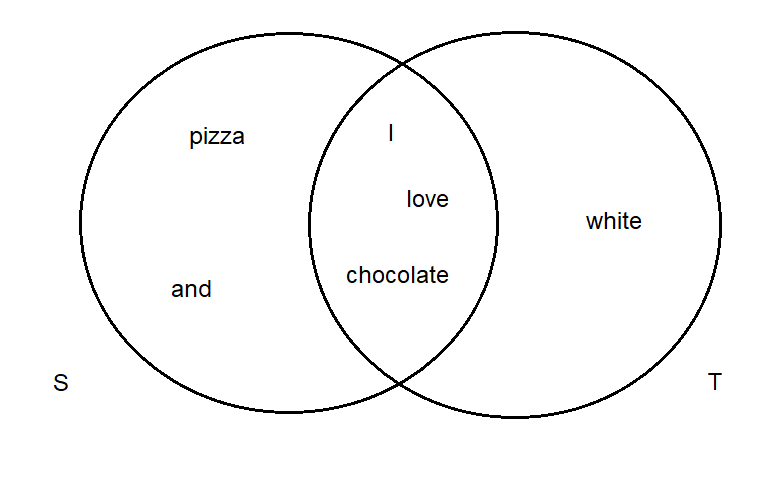
\includegraphics[width=3in]{JaccardExample}
	\label{fig:JaccardExample}
	
	Figure \ref{fig:JaccardExample}: Two sets with Jaccard Index 3/6.
\end{center}

% Falta dir qu� passa si hi ha poques paraules? Fals positiu...?

\end{exmp}

\section{Shingling of Documents}

Any pair of documents can be compared by watching the number of repeated strings they have.
\underline{The more common strings, the more probable is that one is a duplicate from the other.}
One way to represent a document as a set is to insert in the set each string that appears in it. If we do so, then duplicated documents that have reorganized the sentences or even the entire text will have plenty of common strings, and will be detected as duplicated.

\subsection{k-Shingles}

The idea is not to insert in the set all the words, but a set of characters of size \textit{k}. Thus, each element of the set will have the same size as the others.

The question now is how big \textit{k} should be? If we take a small value of \textit{k}, this will result in many shingles that are present in all documents. Suppose we choose the extreme case (\textit{k} = 1). Then, all documents would result to be similar, as the most used characters are present in all documents. However, if we take a big value of \textit{k}, then any pair of documents would not share a shingle.

The value of \textit{k} depends on the size of the documents. A poem will not have the same \textit{k} value than an article. Otherwise, we could have the problems mentioned before.
According to Anand Rajaraman, Jure Leskovec,
and Jeffrey D. Ullman (2011), "k should be picked large enough that the probability of any given shingle appearing in any given document is low." (p. 78).


\section{Compairing Similarity Using The Sets}

If we succeed in shingling the documents by using the \textit{k}-Shingling technique, we will only have to compare all pairs of documents using the Jaccard Index and say if there is similarity between them or not. 
In order to do this, we have to store all the information in a data structure, for instance (\underline{e.g.}), a matrix. By doing this, we have two problems: time and space complexity. $<$= \textbf{Correcte que vagi aqu� la �lima frase?}

\subsection{Matrix Representation}

To represent the matrix, we will put the documents' sets in the columns and the union of all the documents' sets in the rows. The values of the matrix will be the following:
\[
\begin{dcases}
    1,& \text{if column \textit{c} contains row \textit{r}} \\
    0,              & \text{otherwise}
\end{dcases}
\]

�For any pair of row \textit{r} and column \textit{c}, if the set in the colum \textit{c} has the element in the row \textit{r}, the matrix will have a 1 in the cell (\textit{r}, \textit{c}). Otherwise, the cell will have a 0.?

\begin{exmp}
For this example we will use two sets representing the words "Nadal" and "Nadia". Let k = 2 to form the k-Shingles.

\begin{center}
	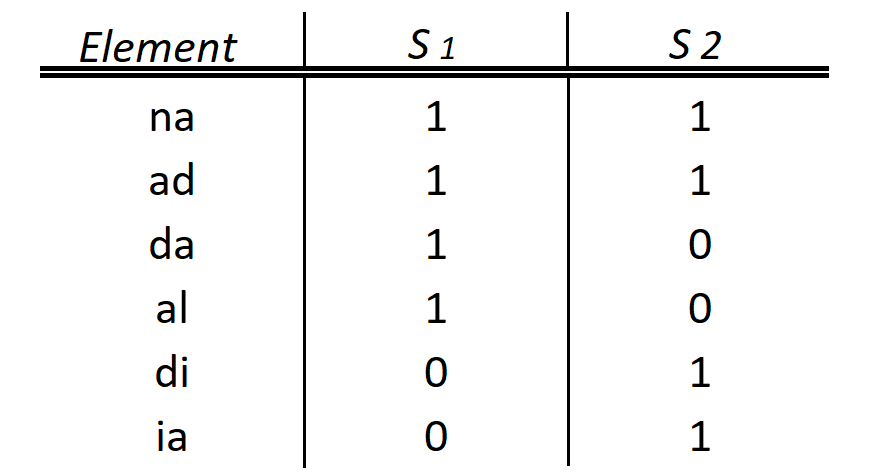
\includegraphics[width=2in]{matrixRepresentation}
	\label{fig:matrixRepresentation}
	
	Figure \ref{fig:matrixRepresentation}: Representation of the matrix with two sets S and T.
\end{center}

\label{exmp:matrixRepresentation}
\end{exmp}

% Parlar de que la probabilitat �s gaireb� la mateixa?

In this type of matrices, for any pair of columns we can have 4 types of results, which are the permutations of 0s and 1s of size 2:

\begin{center}
	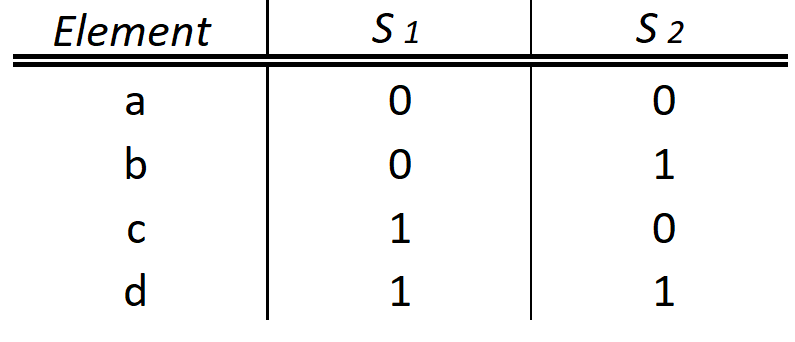
\includegraphics[width=2in]{typesValues}
	\label{fig:typesValues}
	
	\textit{\underline{Figure \ref{fig:typesValues}}: Representation of the matrix with all the possible permutations.}
\end{center}

Note that as the matrix is sparse, most of the rows will be of type \textit{a}. If we try to calculate the similarity between two sets $S_1$ and $S_2$ using the matrix and the Jaccard Index, we will have the following result:

\begin{equation}
J(S_1, S_2) = \dfrac{Q(d)}{Q(b)+Q(c)+Q(d)}
\end{equation}

Where Q(x) is the number of rows of type \textit{x}. Q(d) is the intersection of the sets and Q(b) + Q(c) + Q(d) is the union of the sets.

\subsubsection{Time Complexity}

Imagine we have \textit{n} documents. Then, we have to compare each document with all the rest. Thus, the number of comparisons we have to do is $n*(n-1)/2$ which is equal to $O$($n^2$) �$omega$($n*log(n)$)? O potser �s Theta de $n^2$?.

\begin{exmp}
Suppose we have 1 million documents. The number of comparisons would be $5*10^{11}$ which is a huge number.

\begin{equation}
\dfrac{(1*10^{6})*999.999} {2} = 499.999,5*10^{6} \approx 5*10^{11}
\end{equation}

\end{exmp}

% No s'arregla la time complexity?

\subsubsection{Space Complexity}

In typical applications the matrix is sparse, which means that there are more 0s than 1s. �We can demonstrate this by calculating the \underline{probability} of an element of the set to belong to a document D.?

If we take \textit{k} shingles, then the document have relatively few of the possible shingles.
Another way to think about this is with the toys in Christmas Day. Kids would be the columns of the matrix and toys, the rows. Usually, kids would like to have a specific toy, which is very popular at that moment. Then, lots of toys would not be buyed for any kid.

\subsection{Minhashing}

The main goal using minhashing is to reduce a lot the space complexity. We can achieve this by subsituting the matrix shown before by another matrix called "signature matrix".

Signatures are smaller representations of the sets, but they still preserve the similarity of the sets they represent. We will demonstrate this in the next section.

To minhash a set, first pick a random permutation of the rows. Then, the minhash value is the value of the first row that has a 1, preserving the permuted order.

\begin{exmp}
In this example we will reuse the two sets of Example \ref{exmp:matrixRepresentation}. Suppose that the random permutation has given the following order: "di", "da", "ia", "na", "ad", "al". Let h be the minhash function.

\begin{center}
	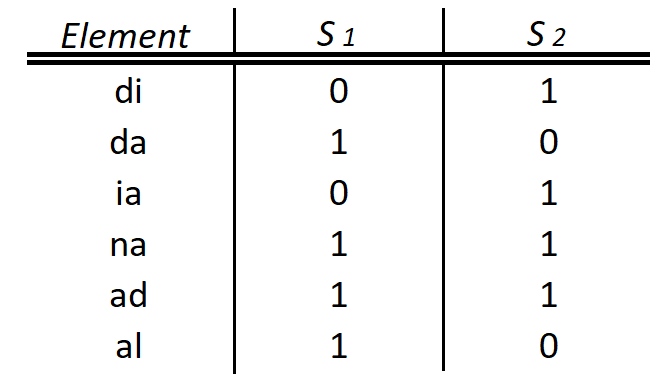
\includegraphics[width=2in]{permutationMatrixSignature}
	\label{fig:permutationMatrixSignature}
	
	Figure \ref{fig:permutationMatrixSignature}: Permutation of the matrix of Example \ref{exmp:matrixRepresentation}.
\end{center}

In the first column, we can see that $h(S_1) = "da"$ and in the second one we see that $h(S_2) = "di"$.

\end{exmp}

With this technique, we can see that every time we do a permutation, we only occupy one new row of the "signature matrix", which is reducing a lot the space.

\subsubsection{Preserving the Jaccard Index}

As we mentioned before, the Jaccard Index in the matrix is equal to the number of rows of type \textit{d} divided by the number of rows of type \textit{b} + \textit{c} + \textit{d}. And that index is preserved in the "signature matrix".

\begin{proof}
Look down through the \underline{permuted columns} $C_1$ and $C_2$ until we see a 1 in any of the two columns. Then, we can have a row of type \textit{b} or \textit{c}, where only one of the columns have a 1, or a row of type \textit{d}, where both columns have a 1 in it.
If we find a row of type \textit{d}, then the minhash function will take the same row. Thus, $h(C_1) = h(C_2)$.
Otherwise, we must have a row of type \textit{b} or \textit{c} and $h(C_1) \neq h(C_2)$.

We can see that this is exactly the Jaccard Index. The probability of two columns have the same minhash value is equal to the number of rows of type \textit{d} divided by the number of rows of type \textit{b} + \textit{c} + \textit{d}.

\begin{equation}
P[h(C_1) = h(C_2)] = J(C_1, C_2)
\end{equation}

\end{proof}

\subsubsection{Optimizing the Time for Permutations}
Encara falta posar cosetes NENG!

\begin{algorithmic}
%\Require $n \geq 0$
%\Ensure $y = x^n$
 \For{each row $r$}                    
  \For{each hash function $h_i$}                    
    \State {compute $h_i(r)$;}
  \EndFor
 \EndFor

 \For{each column $c$}                    
  \If{$c$ has 1 in row $r$}
    \For{each hash function $h_i$}                    
      \If{$h_i(r)$ is smaller than $M(i, c)$}
  	    \State $M(i, c) := h_I(r)$;
  	  \EndIf
    \EndFor
  \EndIf
 \EndFor
\end{algorithmic}

\section{Locality Sensitive Hashing (LSH)}

Mas texto.

\section{Algorithms}

L'objectiu �s mostrar la idea que hi ha darrere els algorismes. No es mostrar� part del codi real. Si es vol mirar el codi, s'haru�n d'anar als arxius corresponents.

\subsection{Jaccard Similarity}

The main objective in this section is to calculate the Jaccard Similarity between two documents in different ways.

\subsubsection{k-Shingles}

The idea is to create two sets, one per document, and insert all substrings of size \textit{k} of the documents. Afterwards, we will just have two make a division: the number of shingles in the intersection divided by the number of shingles in the union.

For each document:

\begin{algorithmic}
 \Require $k$
 \Ensure Returns an unordered\_set with all the substrings of size k of the document
 \State{\textit{words} := entire document}
 \State{\textit{pos} := 0}
 \State{unordered\_set \textit{S} := $\O$}
 \While {\textit{pos + k} $<=$ \textit{words.size()}}
	\State{\textit{sub} := substring from \textit{pos} to \textit{pos + (k - 1)}}
	\State{insert \textit{sub} into \textit{S}}
 \EndWhile
 \State{return \textit{S}}
\end{algorithmic}
\hfill
\hfill
Once we have calculated the \textit{k}-Shingles, we need to compute the intersection and the union of the sets. Note that we insert the substrings in an unordered set. This will be very usefull to improve the time complexity in the next two algorithms:
\hfill
\hfill
\begin{algorithmic}
 \Require Two sets $S_1$ and $S_2$
 \Ensure Returns the intersection set between $S_1$ and $S_2$
 \State{unordered\_set intersection := $\O$}
 \For{each element in $S_1$}                                       
  \If {$S_2$ contains the element in $S_1$}
	\State{insert the element into intersection}
  \EndIf
 \EndFor
 \State{return \textit{intersection}}
\end{algorithmic}
\hfill
\hfill
\begin{algorithmic}
 \Require Two sets $S_1$ and $S_2$
 \Ensure Returns the union set between $S_1$ and $S_2$
 \State{unordered\_set union := $S_1$}
 \For{each element in $S_2$}                                       
  \If {the element in $S_1$ is not contained in $S_1$}
	\State{insert the element into union}
  \EndIf
 \EndFor
 \State{return \textit{union}}
\end{algorithmic}

As you can see, we visit only one set in each algorithm. The good thing is that finding if an element belongs to an unordered set or not is $O(1)$ (IN THE AVREAGE TIME?????). Thus, the time complexity for these two algorithms is $O(n)$, where \textit{n} is the size of the smallest unordered set\footnote{Note that we can change the set we are visiting by the other one. In the intersection, if $S_2$ is smaller than $S_1$, we can visit $S_2$. In the union, if $S_2$ is bigger than $S_1$, we can match the unordered set with $S_2$ and visit $S_1$.}, and the total time complexity is $O(n)$????????????????????, as inserting elements in an unordered set is $O(1)$ (IN THE AVREAGE TIME?????).

On the other hand, if we would have used the predefined functions \textit{set\_intersection} and \textit{set\_union}, we would have needed two ordered set, as it is a precondition of these two functions. Thus, the total cost would have been $O(n * log(n))$.

Finally, we just have to divide the size of the intersection set by the size of the union set (and multiply by 100 if we want a percentage).

\begin{equation}
Jsim(D_1, D_2) = \dfrac{intersection.size()}{union.size()} * 100
\end{equation}

\paragraph{Cost}

The cost of the first algorithm is $O(k * (t - k))$, where \textit{k} is the k-Shingle value and \textit{t} is the size of \textit{words}. As \textit{k} is always a constant, the final cost of this algorithm is $O(k * t - k^2) = O(t)$. The cost of the next two algorithms are $O(n)$, as we have said in the previous section. Finally, the cost of a division and a multiplication is $O(1)$.

Thus, the total cost of calculating the Jaccard Similarity using only k-Shingles is $O(n) + O(t) + O(1) = O(n)$, as usually the number of shingles is much larger than the size of \textit{words}.

\subsubsection{Minhash Signatures}

We know that implementing just k-Shingling is very expensive in terms of size and time (if we want to compare n documents between them, the complexity is $O(n^2)$). Implementing minhash signatures will help on this a lot. However, the Jaccard Similarity will not be the exact value. To do this, we will use as our input the k-Shingle sets calculated in the previous section.
\hfill
\hfill
\begin{algorithmic}
 \Require Two sets $S_1$ and $S_2$
 \Ensure Returns an approximate Jaccard Similarity value between $S_1$ and $S_2$
 \State{unordered\_set union = $S_1 U S_2$}
 \State{matrix signatures = infinity?????????????????????? S'enten que �s cada posici�?}
 \State{vector h = all the hash functions we will use}
 
  \For{each row $r$}                    
  \For{each hash function $h[i]$}                    
    \State {compute $h[i](r)$;}
  \EndFor
 \For{each column $c$}                    
  \If{$c$ has 1 in row $r$}
    \For{each hash function $h[i]$}                    
      \If{$h[i](r)$ is smaller than $signatures[i][c]$}
  	    \State $signatures[i][c] := h[i](r)$;
  	  \EndIf
    \EndFor
  \EndIf
 \EndFor
  \EndFor
 \State{intersection := 0}
 \State{doc1 := 0}
 \State{doc2 := 1}
 \For{each hash function $h[i]$}                    
    \If{$signatures[i][doc1] == signatures[i][doc2]$}
      \If{$signatures[i][doc1] != infinity$}
  	  	\State{++intersection}
  	  \EndIf
  	\EndIf
  \EndFor
 \State{return $\dfrac{intersection}{h.size()}$}
\end{algorithmic}

\hfill

FALTA PARLAR DE LES HASH FUNCTIONS!!!!!!!!!!!!!!!!!!!!!!!!!!!!!!!!!!!!!!!!!!!!!!!!!!!!!!!!!!!!!!!!!!!!!!!!!!!!!!!!!!!!!!!!!!!!!!!!!!!!!!!!!!!!!!

\paragraph{Cost}

We can deduce by just watching the code that the time complexity will come from the first for loop, as it is the one that has to compute most things.
Inside the loop, we have two more loops:

\begin{enumerate}
   \item This loop is responsible of calculating the hash functions taking as the input the row number. Let \textit{h} be the number of hash functions we are using. Then, the cost is $O(h)$ because the calculus done inside this loop is constant.
   
   \item This other loop is the one that updates (or not) the signature matrix. For every column \textit{c}:
   \begin{itemize}
     \item Watch if the set representing the document has the shingle of the row \textit{r}. The cost of doing this is $O(1)$.
     \item Compare the results of all the values computed in the previous for. If any value is smaller than the one that is in the signature matrix at position [\textit{h}][\textit{c}], just replace it by the new value. The cost of this for is $O(c * h)$, where \textit{c} is the number of documents and \textit{h} is the number of hash functions.
   \end{itemize}
\end{enumerate}

Thus, the cost of this function is $O(r * (h + c * (h + 1))) = O(r * h + r * c * h + r * c) = O(r * c * h)$, where \textit{r} is the number of rows and \textit{h} and \textit{c} the values explained before. We should point that \textit{h} is a constant value (usually 200 is correct), so the real cost is $O(r * c)$.

\section{Referencies}

\url{https://towardsdatascience.com/understanding-locality-sensitive-hashing-49f6d1f6134}


\url{https://santhoshhari.github.io/Locality-Sensitive-Hashing/}

\url{https://www.youtube.com/watch?v=96WOGPUgMfw}

\url{https://www.youtube.com/watch?v=_1D35bN95Go}

\url{https://medium.com/engineering-brainly/locality-sensitive-hashing-explained-304eb39291e4}

\url{http://www.mit.edu/~andoni/LSH/}

\url{http://infolab.stanford.edu/~ullman/mmds/ch3.pdf}

\url{https://aerodatablog.wordpress.com/2017/11/29/locality-sensitive-hashing-lsh/}


% Bibliograf�a.
%-----------------------------------------------------------------
\begin{thebibliography}{99}

\bibitem{Cd94} Author, \emph{Title}, Editor, (year)

\end{thebibliography}

\end{document}